\chapter{Interest Driven Content Dissemination Architecture for Disruption Tolerant Networks}
\label{chapter:PTMP}
\minitoc

Mobile networking is quickly reaching a tipping point. While data has been a second-class customer for cellular networks until recently, the wide spread of smart phones, and the access these provide to existing and novel applications, are generating unprecedented amounts of mobile data. The capacity of current cellular infrastructures has already been pushed to the limit~\cite{ATT}. To support the increasing number of devices generating data at high rates, ISPs will inevitably be pushed towards either lowering bandwidth quotas~\cite{ATT}, adopting non flat rate plans, or deploying (expensive) next generation equipment. This has lead many researchers (and industry) to explore alternative or hybrid architectural solutions~\cite{CellOffLoading}.

To this end, direct mobile-to-mobile communication can be leveraged to harvest the large amounts of unused bandwidth between wireless devices in proximity. While multi-hop communication over mobile devices has been recently dealt with in the context of Delay Tolerant Networks (DTNs), increasing user demand for content is creating a shift in focus towards content and data centric systems (e.g. the CCN project~\cite{CCN}), in both wired and wireless Internet. As a result, a number of content dissemination systems have been recently proposed for mobile devices \emph{in the wild} to exchange content of interest in a peer-to-peer manner~\cite{TACODTN, Peoplenet, podnet07, May07wirelessopportunistic, ContentPlace, OptimalChannelChoice, SocialCast, Boldrini:2008:MDD}.

In addition to dealing with the challenging networking conditions, content sharing systems for DTNs have two main functions to perform: \emph{(i)} propagation of interests and content discovery;  \emph{(ii)} delivery of matching content (over one or more hops);
A number of architectural decisions can be made to achieve these goals, leading to publish/subscribe systems~\cite{TACODTN, Peoplenet}, query-based, broker-based~\cite{podnet07, LOCUS, May07wirelessopportunistic, ContentPlace, OptimalChannelChoice, SocialCast, Boldrini:2008:MDD}, etc. These systems aim to maximize the amount of useful content users can receive from the network. Nevertheless, distributed (or peer-to-peer) content sharing systems have one more important goal: \emph{(iii)} \emph{to ensure enough nodes collaborate to make the system interesting to participants.} This goal is often \emph{conflicting} with optimal algorithms for \emph{(i)} and \emph{(ii)}, and has been a major ``deal-breaker'' in most envisioned architectures for mobile ad hoc networks~\cite{NashEquilibria}. Mobile devices are controlled by rational people and we should expect them to behave selfishly by attempting to maximize their revenues and conserve their resources, unless cooperation is somehow incentivized and free-riders penalized.

The following ``architectural dilemma'' arises then when considering a content sharing architecture over \emph{non-altruistic} mobile devices. Nodes can choose to only store and share content they personally consume (thus somewhat mitigating selfish ``inclinations''), and new content of interest can be retrieved from encountered nodes~\cite{podnet07}. This greatly simplifies content discovery and delivery. To further protect nodes against free-riders, a tit-for-tat (TFT) mechanism could be enforced. Yet, this approach is very restrictive: content of interest can be retrieved \emph{only if the set of encountered nodes are also interested in (and carry) the requested content}.
This can lead to long delays and a \emph{suboptimal} query success rate \emph{even if TFT is not used}, if the mobility of nodes with common interests do not coincide.

To improve hit rates, nodes could use their spare resources (contact bandwidth, disk space) to collect, store, and relay additional content, not to be consumed locally~\cite{ContentPlace, SocialCast, OptimalChannelChoice, SocialCast, Boldrini:2008:MDD}. An interesting optimization problem then arises: how should the total spare bandwidth in the network be optimally allocated to available content so as to maximize the overall network hit rate? Answers include randomized or popularity-based local heuristics~\cite{May07wirelessopportunistic}, using this buffer space only for ``friends'' and social peers~\cite{ContentPlace, SocialCast, Boldrini:2008:MDD}, as well as optimal distributed algorithms~\cite{OptimalChannelChoice}. Unfortunately, none of these solutions answers \emph{why} participating nodes should collaborate implementing the policy of choice. In fact, we argue that \emph{this optimization problem needs to be turned on its head, in light of the non-altruistic nature of users.}

Throught this chapter, we propose MobiTrade, an approach that optimizes the content sharing strategy from the perspective of each individual participant, rather than that of the network. First, we argue that Tit-For-Tat (TFT) should be directly employed in order to \emph{(a)} isolate free-riders and \emph{(b)} create incentives for nodes to share their resources. TFT gives content of non-direct interest monetary value. If a node B has content that A is interested in, but A does not have something to give back, A now has the incentive to fetch something for B (perhaps from a remote node that B never encounters). B now retrieves content that would otherwise be inaccessible to it (due to its mobility pattern), and A retrieves content that is easy accessible but that it couldn't ``afford'' before. While TFT is well known both in P2P~\cite{BitHoc} and opportunistic networks~\cite{BarterDTN} communities, it does not answer itself, \emph{how mobile devices should optimally (re-)act in the presence of TFT} towards maximizing their revenues. MobiTrade answers this question by introducing a content utility framework that aims to \emph{maximize the expected future exchange value of the content inventory stored by each node}. Intuitively, the value of a piece of content to a node A should depend on \emph{(i)} how many are interested in it, \emph{(ii)} how often does A see these nodes, \emph{(iii)} how much content, interesting to A, do these nodes have, \emph{(iv)} how ``well-behaved'' are these nodes. MobiTrade uses a simply, robust utility function that implicitly captures all these features, without explicitly measuring each one, that turns each node into a \emph{merchant} fetching the content that has the highest chance to be sold (and exchanged for content of interest) to its good \emph{clients}

Summarizing, the major contributions of this work are the following:
\begin{enumerate}
    \item We formulate the optimal content sharing problem in DTNs from the perspective of non-altruistic nodes and assuming a tit-for-tat mechanism to isolate free-riders.
    \item We propose MobiTrade, a utility-based solution to this problem that predicts the (exchange) value of each piece of content and provides a customized resource allocation strategy for each node, \emph{matched} to each own interests and mobility pattern.
    \item Using a game-theoretic framework and simulations (with both real and synthetic mobility), we show that turning on the MobiTrade mechanism is an \emph{efficient} Nash equilibrium.
\end{enumerate}

To our best knowledge, this is the first content sharing system for DTNs that can both deal with rational, selfish nodes while at the same time achieving good global outcomes \emph{without explicit hard constraints on the topology and dependency of nodes}. 

The rest of this chapter is organized as follow. Section~\ref{MobiTrade-architecture} describes the MobiTrade architecture. Then, we provide a detailed simulation analysis in Section~\ref{performance-evaluation} based on both synthetic~\cite{HCMM} and real mobility traces~\cite{KAIST} and we compare MobiTrade to different content dissemination policies. Finally, we summarize our conclusions and discuss future work in Section~\ref{conclusion}.


\section{MobiTrade Architecture}
\label{MobiTrade-architecture}
\subsection{MobiTrade Data Records}
\label{content-channel-records}

In a content dissemination architecture, nodes need first to somehow express their interests for different (types of) content and advertise these interests. To this end, we borrow the concept of \emph{channels}, introduced in~\cite{May07wirelessopportunistic}. Specifically, the MobiTrade architecture relies on two data records: content and channel records (Figure~\ref{records}).

\emph{Channel Record:} A user asks for a set of contents by creating locally a channel record that encapsulates the set of keywords the user thinks they better describe the contents she is looking for. Channels can be added or deleted by the user, at any time. In contrast to the CCN model~\cite{CCN}, the channel record in MobiTrade is \emph{one-for-many} (not one-for-one). A desirable content is identified based on a match between the channel keywords and the content description (also characterized by a set of keywords). We think that such a match process is more appropriate for the communication model we are proposing, where the user might not know the exact content he is looking for, or might anyway be interested in all contents matching the description (e.g. Madonna songs, photos of Nice, sports tickets for sale). 

A lot more can be said about this channel structure (e.g. hierarchies, merging and splitting of channels, semantic content matching, etc.), but this is beyond the scope of this paper. Instead, we choose to use a simple channel structure here and focus on the algorithmic part of the system. Finally, each channel record contains a \emph{utility} entry. This is a key quantity for MobiTrade, allowing our system to optimize various important functions (scheduling, inventory management, collaboration profiling, etc.). For now, we will assume this as given, but Section~\ref{managing-channels} is devoted to how this utility is derived.

\emph{Content Record:} In addition to the content description, a content record contains a number of additional fields. First, we associate to each MobiTrade content a $TTL$ (Time to Live). By the end of this time, records can be removed. The cases requiring this $TTL$ field are many, for example someone could be interested in selling something today. To ensure devices respect this $TTL$ field, MobiTrade devices do not reward each other for expired content.

\begin{figure}[!h]
\centering
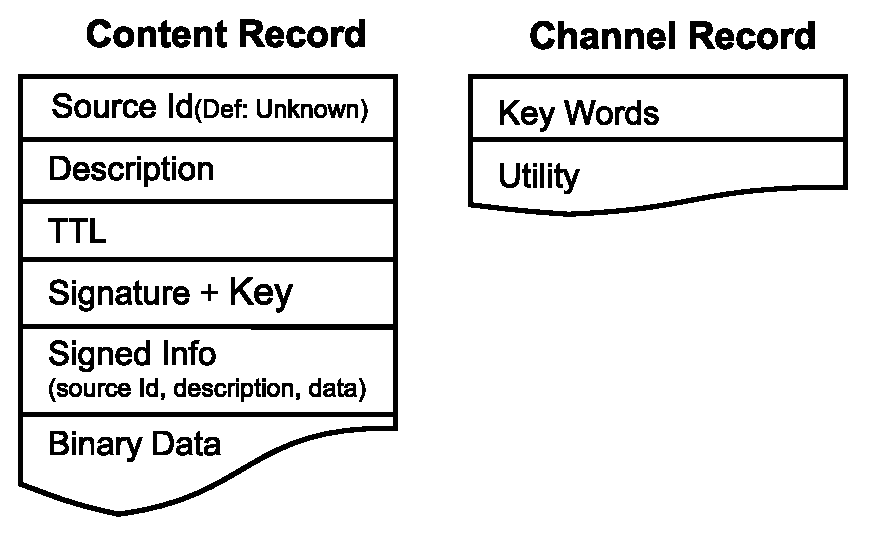
\includegraphics[width=2.5in,height=2in]{Chapitre5/ContentsInterestsRecords.eps}
\vspace{-0.1in}
\caption{MobiTrade data records and channel storage}
\label{records}
\vspace{-0.2in}
\end{figure}

Furthermore, to provide users with a full control over their privacy (i.e., the contents they publish and their center of interests), we choose to keep anonymous any generated channel record (no user or device ID are stored). Nevertheless, for contents, one still has the possibility to associate to them a \emph{canonical} source name that refers in some way to the content publisher. This field does not correspond necessarily to the user device address, but it can hold the publisher postal address or its phone number, which can be used for distinguishing between contents, feedback mechanisms on separate communication mediums or authentication purposes.

Finally, to provide for some MobiTrade security, we choose to use a CCN like \emph{content-based security} model~\cite{CCN}. With this model, protection and trust travel with the content itself, rather than being a property of the connections over which it is transmitted.
MobiTrade devices authenticate via the signature field (Figure~\ref{records}), the binding between the content source ID, its description and some parts of its data. In addition to this signature, each signed MobiTrade content carries with it the public key necessary for its verification by other devices. The signature algorithm can be selected to meet the performance requirements of that particular published data.

\subsection{MobiTrade Protocol}
\label{communication-protocol}

Communication within the MobiTrade architecture is driven by the consumers of contents. A user asks for contents by ``joining'' a channel to which these might belong, storing the respective record(s) locally on the device until it becomes out of date. Then, each time a new meeting opportunity arises with another mobile device, both devices initiate the MobiTrade communication protocol that has two main functions:
\begin{itemize}
\item (\emph{Fair Content Exchange}) to help nodes identify content of interest in their peer's inventory (buffer) and provide a set of rules to exchange such content in a \emph{fair} manner.
\item (\emph{Inventory Management}) to allow nodes to profile each exchange (\emph{learning}) and use this knowledge to improve the outcome of future interactions (\emph{prediction}).
\end{itemize}

The MobiTrade protocol is summarized in Figure~\ref{protocol}. Each device starts by sending its list of channels to the other device. Based on it, each device decides on the set of contents to forward, i.e. content in its buffer matching one of the channels requested by its peer. These contents are scheduled for transmission and passed to the \emph{Tit-For-Tat (TFT)} trading algorithm (Section~\ref{contents-trading-scheduling}) that ensures an equitable exchange.

In addition to channels the node is personally interested in, if extra space is available, it might choose to join ``foreign'' channels. Content for these channels is not stored for personal consumption, but can be used as exchange currency during the TFT phase, in order to acquire additional content of interest. This provides the incentive to nodes to act as \emph{merchants}, collecting and carrying content to be used only for trading. This also allows content to \emph{propagate efficiently across the network and between remote producer-consumer pairs, without any explicit routing mechanism}. %From the perspective of the MobiTrade protocol, own and foreign channels are equivalent.

After content starts being exchanged (one-by-one), a node receiving a content might need to perform some inventory management. First, if it already has this piece of content (or the content is expired), it will drop it\footnote{This is possible, since nodes only send to each other lists of channels and not a detailed list of contents. This is a coding trade-off that tries to avoid large amounts of meta-data being exchanged before any actual content is sent. On the other hand, it might also lead to some wasted bandwidth if lots of duplicate content is transmitted. A possible middle-ground solution to this problem could be the use of Bloom filters.}. If the content is new, and there is available buffer space for the channel this belongs to, the content is stored in the buffer. The exchange finishes once the transfer of the requested contents ends or the two devices get out of the range of each other. At this point, both devices update the set of channels they are keeping track of as well as their corresponding utilities based on the (profiled) outcome of the session (as explained in Section~\ref{managing-channels}).

\subsection{Proportional Storage and Bandwidth Allocation}
\label{buffer-management}

In a context with many nodes, various channels, and lots of multimedia content, node buffers will be operated most of the time at capacity and contact duration between nodes might not suffice to exchange all intended content. This highlights the need for efficient resource allocation algorithms. Unlike related work~\cite{ContentPlace}~\cite{May07wirelessopportunistic}, \emph{MobiTrade allocates both buffer space and contact bandwidth in an equitable way among the different channels.}

First, MobiTrade implements a mechanism of \emph{proportional soft quotas} to share available buffer space among channels. Let a node carry $N$ channels with channel utilities $U(i), i \in \{1,N\}$, and have a total buffer capacity of $B$. Then, the \emph{quota} $B(i)$ of the buffer space channel $i$ is entitled to is
\begin{eqnarray*}
B(i) = \frac{U(i)}{\sum_{i} U(i)} B.
\end{eqnarray*}
The proportion of storage allocated to a channel is proportional to its utility. Quotas are updated whenever one or more of the channel utilities change or channels are added/removed.

Based on these quotas and the amount of storage channel $i$ is \emph{currently} occupying, let $S(i)$, a node receiving a content (of $W$ bytes) for channel $i$ will perform the following actions:
\begin{itemize}
\item if $S(i) + W < B(i)$, then store the content.
\item if $S(i) + W > B(i)$ and $\sum_{i} S(i) + W < B$, then store content.
\item if $S(i) + W > B(i)$ and $\sum_{i} S(i) + W > B$, then pick the channel $j$ maximizing $\max_{j} (S(j) - B(j))$ and drop the oldest content for this channel.
\end{itemize}
Points (2) and (3) above imply that the quotas $B(i)$ are soft. Channels can exceed their share and take over free space, if any is available. However, as soon as the buffer is full, the policy pushes shares back to their just proportion.

Finally, in the presence of limited contact durations, a device cannot simply forward contents by decreasing order of the utilities of their channels since a channel can match more than one content. For example, a MobiTrade device can face a situation where many contents match a popular channel, and hence it keeps forwarding only those contents at the expense of other channels which are less popular. To remedy this, MobiTrade applies the \emph{Weighted Fair Queuing} policy which prevents starvation of channels and ensures that contents are forwarded proportionally to the utility value of the channel they match. 

As a final note, when the scheduling policy decides to forward a set of contents from the same channel, MobiTrade sends the \emph{youngest} contents first. This decision is motivated by our findings in~\cite{TMC:Report} and is complementary to the drop oldest policy applied among the contents of the same channel in case of congestion. More sophisticated policies could be also applied~\cite{TMC:Report}, but this is beyond the scope of this paper.

\begin{figure}[!h]
\centering
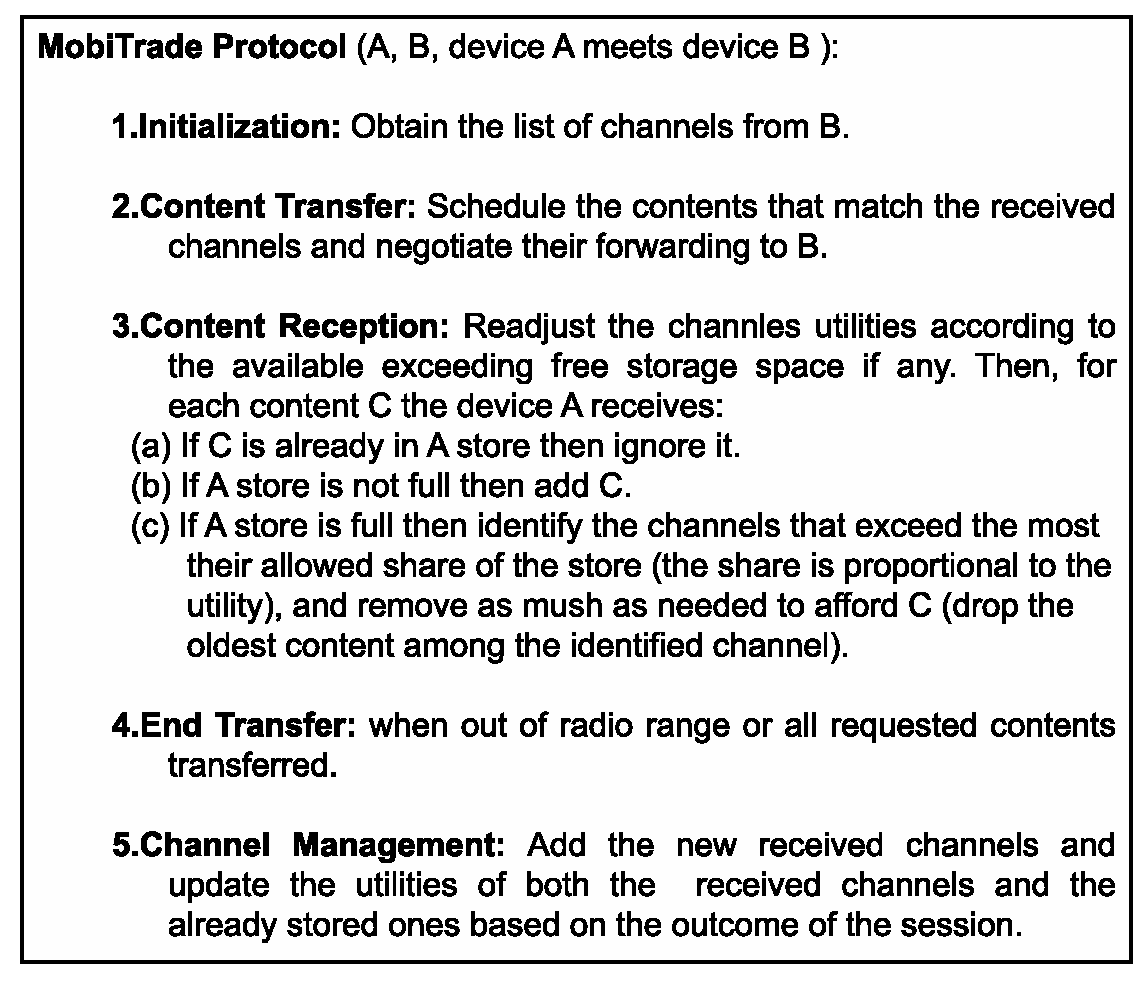
\includegraphics[width=3.5in,height=3in]{Chapitre5/MobiTrade-Protocol.eps}
\vspace{-0.1in}
\caption{MobiTrade protocol}
\label{protocol}
\vspace{-0.1in}
\end{figure}

\subsection{Tit-For-Tat Trading}
\label{contents-trading-scheduling}

One major difference of our system compared to other content dissemination solutions for DTNs (e.g.~\cite{May07wirelessopportunistic,ContentPlace,TACODTN}) is that we assume that participating users are selfish by default. Thus they might act as free-riders: during a meeting they receive content they want but don't give something back (even if they have), in order to save transmission power or to save some bandwidth. Or, they might not collect content their peers are requesting. Experience teaches us that even in the absence of power or storage concerns (e.g. wired users of BitTorrent), additional concerns (legal, malice), might motivate users to circumvent collaborative mechanisms~\cite{BitThief}. We believe these are \emph{powerful incentives that could sabotage any collaborative content dissemination system, if not properly handled}.

In order to remedy this and isolate selfish users, a \emph{strict} Tit-For-Tat (TFT) trading is enforced during meetings. Content scheduled for exchange is forwarded one-by-one (or in equally sized blocks/pieces, if contents are not of equal size), i.e. node A sends some, then node B sends some, then node A again, etc. Forwarding of content stops when the other device cannot (or chooses not to) reciprocate the amount of bytes it received\footnote{In order to solve the bootstrapping issue, when two well-intended devices meet for the first time, MobiTrade enables generous cooperation up to a certain amount as described in Section~\ref{managing-channels}.}. 

In addition to this TFT mechanism ensuring that selfish nodes are not serviced when content for them \emph{is} available, a utility maintenance mechanism (to be described in Section~\ref{managing-channels}) further ensures that well-intended nodes will not waste their resources collecting content for selfish nodes from which they will not receive any reward.


\section{Inference of Channel Utility}
\label{managing-channels}

MobiTrade aims at maximizing the number of collected contents while providing incentives for devices to collaborate. To have their requests satisfied, MobiTrade devices have to propose contents to other devices in counterpart of what they are looking for. As said before, each device is equipped with a storage space that is filled with contents from the different existing channels, which are used later as trading currency. This storage space is filled so as to satisfy the future demand: each channel occupies a proportion of the storage equal to the reward it is expected to bring upon future meetings. Due to Tit-For-Tat trading, the reward from carrying a channel is the amount of data from this channel a device will sell upon future meetings (to get both data for its own usage and data used for later trading). Hence, \emph{to optimize performance, MobiTrade devices should be able to quantify the expected reward from the channels they carry.}

In MobiTrade, the expected reward from each channel is modeled through a utility function used for ranking contents upon a meeting and for dropping them upon saturation of the storage. In this section, we detail how these utilities are calculated. Table~\ref{table:notation} summarizes some useful notation.

\begin{table}
\vspace{-0.1in}
\caption{Notation}
\centering
\label{table:notation}
\footnotesize
\begin{tabular}{|p{2cm}||p{10cm}|}
\hline
\bfseries Variable & \bfseries Description\\
\hline
$U_{CH}(n)$ & In bytes. Models the utility of the channel $CH$ at the $n_{th}$ meeting.\\
\hline
$X(CH)$ & 0 or 1. Expresses whether the met device is also interested in channel $CH$ or not.\\
\hline
$CL(CH)$   & In bytes. Expresses the collaboration level of the met device during a given meeting with respect to the channel $CH$.\\
\hline
$SC(CH)$   & In bytes. Expresses the number of bytes sent to the met device during a given meeting with respect to the channel $CH$.\\
\hline
$\omega$ & Between 0 and 1. A weight that decides on the elapsed time window over which we average the utility of channels.\\
\hline
$\alpha$ & In bytes. Expresses MobiTrade device generosity level, used to de-block the situation when two devices meet for the first time and request new channels.\\
\hline
$\beta$ & In bytes. Controls the speculation that a MobiTrade device makes regarding the expected future reward from a given channel.\\
\hline
\end{tabular}
\end{table}

For each channel $CH$, MobiTrade defines its utility $U_{CH}(n)$ at the $n^{th}$ meeting (counted over all devices) in a way to reflect the \emph{expected} number of bytes the device will sell from this channel (and thus the bytes of interest these will buy back) with any random device it will meet\footnote{Note that MobiTrade does not differentiate between own and foreign channels (these could also overlap) at the level of calculating utilities. However, foreign content doesn't interfere with content for own consumption. If a peer has content of interest for own consumption, this will always be retrieved, provided it can be ''bought'', and passed to the application. MobiTrade only decides whether this should be further cached in the content storage for future trading.}. This is clearly a complex interplay of mobility patterns, available channels and content, and node interests. \emph{We choose to keep our framework as assumption free as possible about mobility and interest patterns}, and take the following approach.

\noindent \textbf{Calculation and update of channel utilities:}
Assuming stationarity of the network over at least a time window of $2T$, the expected reward from carrying a channel $CH$ can be calculated by averaging all experienced rewards over all meetings in the past time window $T$. Meetings that do not request channel $CH$ count as zero. To facilitate implementation, an Exponential Weighted Moving Average (low pass) filter is used for averaging.

Let's consider a device $A$ and let's suppose that an $(n+1)^{th}$ meeting opportunity arises. After the establishment of the physical connection, both devices exchange matching contents while applying the Tit-For-Tat trading algorithm (as in Figure~\ref{protocol}). Once done, they both record the volume of exchanged data and update each the utilities of the channels they carry. For device $A$ and channel $CH$, this update is done as follows:
\begin{eqnarray*}
U_{CH}(n+1) = \omega . U_{CH}(n) + (1 - \omega) . X(CH) . CL(CH),
\label{eq:utility-updating}
\end{eqnarray*}
where $\omega = (t_{n}-t_{n-1})/T$ is the weight associated to the low pass filter\footnote{By making it function of the elapsed time between the current meeting and the previous one, one can ensure an averaging over a time window $T$.}. Concerning the term on the right hand side, it models the amount of data exchanged with the met device $B$ from channel $CH$. $X(CH)$ is a binary variable that expresses whether $B$ is interested or not in $CH$. This variable captures the popularity of a given channel over all MobiTrade devices met by $A$. As for $CL(CH)$, it captures the volume of contents that could be sold to device $B$ in the future (i.e. a prediction of $B$'s future demand for $CH$).

This calculation leads to several nice properties. First, this utility calculation is per channel and does not account for the physical addresses of encountered devices. The same device met several times or different devices met the same number of times count the same from the viewpoint of MobiTrade, as long as the amount of data sold was the same. This avoids tracking individual devices which improves the scalability of MobiTrade. Second, it does not try to over-optimize for the next meeting only (as could be the case with detailed mobility prediction) but rather optimizes the inventory over a larger time horizon, enough to absorb prediction inaccuracies at individual meetings. Finally, coupled with the Tit-For-Tat algorithm, our utility (through $CL(CH)$) accounts for the collaboration of devices in addition to the popularity of channels. In lack of this feature, a channel widely requested among a group of users, who do not collaborate by bringing back interesting contents for $A$, could force $A$ to keep collecting contents matching $CH$, only to discover later that this content buys him nothing. The storage of $A$ could have been better used by carrying contents for less popular channels but more collaborative devices.

\noindent \textbf{Collaboration and Bootstrapping:}
The $CL(CH)$ term above expresses the collaboration level of the device $B$ with respect to the channel $CH$. If a channel however is requested for the first time at the $(n+1)^{th}$ meeting, its $U_{CH}(n)$ would be initialized to zero. A new node that asks for a channel $CH$, would see its request being ignored, as no content for $CH$ was exchanged in this round. Clearly, an appropriate bootstrapping mechanism is needed, in order to avoid this chicken and egg problem for new nodes or channels. This can be implemented as some \emph{slack} or \emph{generosity} in the $CL(CH)$ calculation and the TFT mechanism. At the same time, this generosity should be such that it \emph{cannot be exploited} by selfish nodes. The calculation of $CL(CH)$ below is inspired from TCP slow start, and attempts to best satisfy the above two (conflicting) goals:

$$
CL(CH) = \left\{
    \begin{array}{ll}
        Max(\alpha, 2 . SC(CH)) & \mbox{if } SC(CH) < \beta, \\
        SC(CH) + \alpha & \mbox{otherwise.}
    \end{array}
\right.
$$
The collaboration level $CL(CH)$, that is, the prediction of future demand, is thus a function of the actual (last exchange) demand $SC(CH)$. If $SC(CH)$ is less than some threshold $\beta$, we allow $SC(CH)$ to double, to accelerate the collaboration process at its beginning; otherwise, devices will have to meet more often to reach a satisfactory collaboration level. After $\beta$\footnote{We take an optimistic approach and choose it equal to the maximum utility value over all channels of $A$.}, the generosity of device $A$ switches into a linear mode when it believes it has successfully approximated the steady-state demand, and only speculates an additional $\alpha$ to $SC(CH)$.

The same factor $\alpha$ is equally used as minimal value for $CL(CH)$ to unblock the situation when device $B$ asks for a new channel ($SC(CH)$ equals zero in this latter case). If a channel does not bring the expected reward for any reason (lack of collaboration, oldness of the contents carried, etc.), this will be reflected by a decrease in $SC(CH)$, which automatically leads to a decrease in the utility value we associate to this channel. Similarly, $\alpha$ also serves to keeps selfish nodes in control. If some selfish device asks for a long list of new channels, MobiTrade will associate initially a small utility value to them. A selfish/malicious user is then obliged to collaborate in order to increase the utilities of his channels and thus the portion of content storage these are given.

From the perspective of a collaborative trader node, a community of non collaborative users is equivalent to a community of users not requesting channels. We believe this improves the robustness of the system and allows it to scale to large networks, without the need for explicit blacklisting and reputation systems (at least for selfish nodes).

%Another feature of setting $CL(CH)$ this way is the ability to protect collaborative users from non collaborative ones. Indeed, a selfish user requesting channels but not collaborating with the other devices will see its $SC(CH)$, and hence its $CL(CH)$, set to low values. The result will be almost equivalent to this user not requesting any channel ($X(CH)$ set to zero). 

\section{Performance Evaluation}
\label{performance-evaluation}

We move now to performance evaluation of our system. We first describe our experimental setup, and then present simulations results for two main types of scenarios: collaborative scenarios and scenarios including selfish users.

\subsection{Experimental Setup}
\label{experimental-setup}

\emph{Protocols:} We have implemented the MobiTrade content dissemination protocol in the NS3 simulator~\cite{NS3}. Throughout our simulations we will be considering two versions of MobiTrade, with (\textbf{MobiTrade + TFT}) and without Tit-For-Tat (\textbf{MobiTrade - TFT}). Note that this corresponds only to the forwarding module, described in Section~\ref{contents-trading-scheduling}. The channel utility maintenance, described in Section~\ref{managing-channels}, is kept on in all scenarios. We have also implemented two different versions of the \emph{podnet07} scheme as a baseline for comparison\footnote{We choose the PodNet framework, as it is the most directly comparable to our scheme, and consists of simple enough mechanisms that we consider practical for implementation. For example, \cite{OptimalChannelChoice} is considerably more complex and based on an MCMC framework that requires careful simulated annealing and might take a long time to converge. Furthermore, \cite{ContentPlace} requires explicit knowledge of social network links, not available in our framework.},  as described, to our best understanding in~\cite{May07wirelessopportunistic} and~\cite{Podcasting:Secon07}: (i) non-collaborative Podcasting, where users just carry and share their own channels~\cite{May07wirelessopportunistic} (\textbf{Podcasting}); (ii) collaborative Podcasting with the \emph{Uniform} channel sharing strategy, where, a device records all channels it has seen in the past and solicits contents for these channels randomly~\cite{Podcasting:Secon07} (\textbf{Podcasting + Uniform}). This latter strategy was shown to perform best in~\cite{Podcasting:Secon07}, compared to other heuristics taking into account channel popularity. As a final note, we stress that MobiTrade's first goal is not to compete with optimal collaborative schemes, but rather to efficiently deal with selfish nodes, without compromising the socially optimal (collaborative) performance.

\emph{Mobility Models:} To evaluate the different protocols, we use two type of mobility scenarios, a state-of-the-art synthetic mobility model (HCMM)~\cite{HCMM} and a real mobility trace (KAIST)~\cite{KAIST}. HCMM is a mobility model inspired by Watts' Caveman model that was shown to reproduce statistics of human mobility, such as inter-contact times and contact duration. In HCMM, the Caveman model is used to define a graph (overlay) with nodes divided into (well connected) groups and each group is assigned to a physical home location. Also, some users belonging to different groups can have links to each other (bridges). These (intra- and inter-group) links are used in HCMM to drive movements: each user moves towards a given group's home location with a probability
proportional to the weight of its links towards the group. In our scenario, we consider 50 users distributed into 5 groups. The plane is divided into a 10*10 grid of cells (5000 m wide), and each cell can serve as a home location for a group.

The KAIST scenario consists of real human mobility traces collected from a university campus (KAIST) in South Korea~\cite{KAIST}. We consider a sample of the KAIST campus traces taken from 50 students, where the GPS receivers log their position at every $30$ seconds. We integrated both mobility models in NS3. Both case studies consist of simulations that last $24$ hours where devices use the $802.11b$ protocol to communicate with a transmission range around $60$ meters.

\emph{Traffic Model:} Unless otherwise stated, each user joins randomly $2$ channels at the beginning of the simulation. For simplicity, we assume that all generated contents have the same size\footnote{Variable sized content could still be split to equal sized pieces or blocks. We defer the study of more complex content structures to future work.}. However, different channels do not need to have the same size (the size of a channel is equal to the sum of its contents' sizes). Some channels might have lots of content, and others less. Finally, we consider that each user generates contents periodically that match one of the channels that were requested by users from other groups\footnote{The content generation interval depends on the number of contents for a channel and the duration of the simulation.}.

\subsection{Collaborative scenarios}
\label{collaborative-scenario}

We first evaluate MobiTrade, assuming all nodes are collaborative, using the following four scenarios (described in Table~\ref{table:c-sim-sce}) (there are $50$ channels in total): {$\mathbf{SC_1}$} implements a \emph{homogeneous traffic} pattern, i.e. each channel has the same size and each user joins the same number of channels. In $\mathbf{SC_2}$, users choose a \emph{random number of channels} to join, but channels still have the same size. In $\mathbf{SC_3}$, users ask for the same number of channels but these have \emph{random sizes}. Finally, $\mathbf{SC_4}$ introduces some \emph{churn}, where $10$ of the users join the simulation after $8$ hours, while existing sessions are ongoing, and leave again $8$ hours later. Due to space limitations, for all scenarios, we show plots for the HCMM mobility model, accompanied with respective results for the KAIST trace summarized in Tables.

\begin{table}[!h]
\vspace{-0.1in}
\caption{Collaborative simulation scenarios}
\centering
\label{table:c-sim-sce}
\footnotesize
\begin{tabular}{|p{3cm}|p{2cm}|p{2cm}|p{2cm}|p{2cm}|}
\hline
\bfseries Sim. Scenario: & $\mathbf{SC_1}$ & $\mathbf{SC_2}$ & $\mathbf{SC_3}$&  $\mathbf{SC_4}$ \\
\hline
\bfseries Nbr. of Users: & 50 & 50 & 50 & 40 + 10 transient\\
\hline
\bfseries Requested CH(s) per User & 2 & random [1, 20]& 2& 2\\
\hline
\bfseries Size of CH(s) (\# of contents) &20  &20 &Random [1, 20]&20 \\
\hline
\end{tabular}
\end{table}

\noindent \textbf{Effect of TTL:} Before we proceed, we take a quick look first into the impact of content TTL. As explained in Section~\ref{MobiTrade-architecture}, our buffer drop and scheduling policies give priority to younger messages\footnote{Note that this age \emph{only} corresponds to the time the content was inserted in the network by its publisher, and does not (directly) relate to the actual age (e.g. an old vs. a new rock song.)}. This is not only in accordance with our daily experience (for many types of content, e.g. news feeds, we prefer to have the most recent version), but has also been shown to be an efficient resource allocation policy in the context of a single channel~\cite{TMC:Report} (intuitively, older content has a higher chance to have been delivered already). Figure~\ref{DO} depicts the MobiTrade average delivery rate as a function of the content $TTL$ (for scenario $\mathbf{SC_1}$), with and without prioritizing younger messages (per channel). It is evident that the higher the (application chosen) $TTL$ the more old content ``hogs'' node buffer and contact bandwidth, not allowing new content to reach its audience. When prioritizing younger messages, not only does performance stabilize, but with an infinite TTL the gain from just this mechanism is up to $76\%$.

\begin{figure}[!h]
  \begin{center}
    \includegraphics[width=3in,height=2.2in]{Chapitre5/fig3.eps}
  \end{center}
  \caption{Drop and Scheduling policy inside the same channel ($\mathbf{SC_1}$).}
  \label{DO}
\end{figure}

\begin{figure}[!h]
  \begin{center}
    \includegraphics[width=3in,height=2.2in]{Chapitre5/fig5.eps}
  \end{center}
  \caption{Fixed number of channels per user and fixed channel size ($\mathbf{SC_1}$).}
  \label{CS+FNC+FCS}
\end{figure}

\noindent \textbf{Scenario} $\mathbf{SC_{1}}$: Figure~\ref{CS+FNC+FCS} compares the performance of MobiTrade with and without TFT and the two versions of Podcasting described in Section~\ref{experimental-setup}. The figure of merit is, again, the average delivery rate, defined as the \emph{amount of content received for channels a node requested} divided by the \emph{total amount of content generated for these channels} (throughout the simulation). This is averaged over all nodes. Delivery rate is plotted as a function of node storage.

There are three main observations to be made in Figure~\ref{CS+FNC+FCS}. \emph{First}, collecting and sharing foreign channels (\textbf{MobiTrade} and \textbf{Podcasting + Uniform}) improves performance compared to only storing own channel. This confirms the findings of~\cite{Podcasting:Secon07}. \emph{Second}, the uniform sharing policy~\cite{Podcasting:Secon07} is clearly not optimal (as suggested also in~\cite{OptimalChannelChoice}), and is significantly outperformed by MobiTrade's inventory management (by up to $2 \times$). This is more pronounced as storage is increased. \emph{Third}, using Tit-For-Tat (TFT) in a context where \emph{all} nodes are well-intended results in a small drop of the average delivery rate by about $6\%$, compared to the case without TFT. Using game theoretic terms, in Section~\ref{game}, we show that \emph{rational users will choose to pay this price to secure themselves from selfish users}. Finally,  Table~\ref{table:kaist:col}, summarizes the respective results for the KAIST trace (we only show values for a buffer of $110$ contents; the plot trend is similar to Figure~\ref{CS+FNC+FCS}). The results for the KAIST trace (row 1) corroborate the above findings.

\begin{figure}[!h]
  \begin{center}
    \includegraphics[width=3in,height=2.2in]{Chapitre5/fig4.eps}
  \end{center}
  \caption{Scenario $\mathbf{SC_2}$.}
  \label{CS+RNC+FCS}
\end{figure}

\begin{figure}[!h]
  \begin{center}
    \includegraphics[width=3in,height=2.2in]{Chapitre5/fig7.eps}
  \end{center}
  \caption{Scenario $\mathbf{SC_3}$.}
  \label{CS+FNC+RCS}
\end{figure}


\begin{table}[!h]
\vspace{-0.1in}
\caption{Avg. delivery rate based on the real KAIST trace (collaborative scenario, content storage size = 110 contents).}
\centering
\label{table:kaist:col}
\footnotesize
\begin{tabular}{|p{3cm}|p{2cm}|p{2cm}|p{2cm}|p{2cm}|}
\hline
\bfseries Policy:& \bfseries MobiTrade + TFT & \bfseries MobiTrade - TFT & \bfseries Podcasting & \bfseries Podcasting Uniform\\
\hline
\bfseries Scenario $\mathbf{SC_{1}}$ & 0.83 & 0.89&0.6 &0.72\\
\hline
\bfseries Scenario $\mathbf{SC_{2}}$ & 0.78 &0.86 &0.75 &0.69\\
\hline
\bfseries Scenario $\mathbf{SC_{3}}$ &0.79  &0.88 &0.68 &0.74\\
\hline
\end{tabular}
\end{table}

\noindent \textbf{Scenarios} $\mathbf{SC_{2}}$ and $\mathbf{SC_{3}}$: These two scenarios consider the effect of heterogeneity with respect to channel demand ($\mathbf{SC_{2}}$) and channel size ($\mathbf{SC_{3}}$). The goal is to examine whether \emph{asymmetry} of demand or supply of content (common in practice) could give rise to \emph{deadlocks} due to the \emph{inherent symmetry} of the Tit-For-Tat mechanism.

Figures~\ref{CS+RNC+FCS} and~\ref{CS+FNC+RCS} show the respective delivery rate for these two scenarios, as a function of storage space. As we can see, traffic asymmetry does not affect the main observations made in scenario $\mathbf{SC_{1}}$. Interestingly,  for ($\mathbf{SC_{2}}$), Podcasting only own channels seems to outperform uniform sharing of foreign channels. Results for the KAIST trace are again in agreement (rows 2 and 3 of Table~\ref{table:kaist:col})). We conclude that, even in the presence of asymmetric traffic, MobiTrade performs up to almost $2\times$ better even without selfish nodes. Finally, while it is clear that these two scenarios do not suffice to \emph{exclude} every probability of a deadlock, they constitute positive evidence to the robustness of MobiTrade. We defer an analytical treatment of deadlocks to future work.


\noindent \textbf{Scenarios} $\mathbf{SC_{4}}$: The objective of this last scenario is to study the impact of \emph{node churn} and the ability of MobiTrade to efficiently bootstrap new nodes. Here, $10$ new users join the simulation after $8$ hours, each one of them asks for $2$ already existing channels, then, it leaves the simulation $8$ hours later. Figure~\ref{10-new-users} plots the average delivery rate among the $10$ new users and the $40$ existing ones as a function of time.
It is evident there, that when the new set of users join already existing channels, they are not blocked. Instead, they are able to collaborate and quickly scale up their performance\footnote{The important thing in this plot is the slope of the curves for new and old nodes, which matches, implying that both types get 
similar service. They differences in absolute value are only because nodes joining late have already missed part of the content already generated for this channel (and possibly dropped due to congestion).}.

\noindent \textbf{Delay:} Finally, in Figure~\ref{avg-delay}, we look at the average delivery delay of different schemes (scenario $\mathbf{SC_{1}}$), measured as \emph{time a matching content is received} $-$ \emph{time it was inserted in the channel}. We can clearly see that the ranking of schemes in terms of delay is similar to the one for delivery ratio (Figure~\ref{CS+FNC+FCS}).

\begin{figure}[!h]
  \begin{center}
    \includegraphics[width=3in,height=2.2in]{Chapitre5/fig8.eps}
  \end{center}
  \caption{Scenario $\mathbf{SC_4}$, 10 new users ask for already existing channels.}
  \label{10-new-users}
\end{figure}

\begin{figure}[!h]
  \begin{center}
    \includegraphics[width=3in,height=2.2in]{Chapitre5/fig12.eps}
  \end{center}
  \caption{Scenario $\mathbf{SC_1}$, studying the average delivery delay.}
  \label{avg-delay}
\end{figure}

\subsection{Scenarios with selfish users (SU)}
\label{selfish-scenario}

Having established the good performance of MobiTrade in the absence of selfish nodes, we now turn our attention to scenarios where few or more nodes might not reciprocate for content they receive. We deem such scenarios as the norm rather than the exception in the real world. As mentioned earlier, most related proposals do not deal (explicitly) with such users. We consider two such scenarios, as described in Table~\ref{table:m-sim-sce}: In $\mathbf{SS_{1}}$, we consider $10$ selfish users among $50$ that ask for different channels than those requested by the remaining collaborative users. In $\mathbf{SS_{2}}$, we consider the same number of selfish users which ask randomly for channels already requested by collaborative users. Selfish users and Collaborative users are denoted with ``SU'' and ``CU'', respectively.

\begin{table}[!h]
\vspace{-0.1in}
\caption{Simulation scenarios including selfish users.}
\centering
\label{table:m-sim-sce}
\footnotesize
\begin{tabular}{|p{3cm}|p{4cm}|p{4cm}|}
\hline
\bfseries Sim. Scenario: & $\mathbf{SS_1}$ & $\mathbf{SS_2}$\\
\hline
\bfseries Nbr. of Users: & 40 CU + 10 SU & 40 CU + 10 SU\\
\hline
\bfseries Nbr. of CH(s) & CU: 2/20 - SU: 2/10 (SU and CU channels differ) & CU, SU: 2/20 (among same channels) \\
\hline
\bfseries Size of CH(s) & CU: 20 - SU: 40  & CU, SU: 20 \\
\hline

\end{tabular}
\end{table}

\noindent \textbf{Scenario} $\mathbf{SS_1}$:  Figure~\ref{SS-Scenario-1} depicts the average delivery rate (for different user strategies, CU and SU) with and without the TFT mechanism enabled. At high congestion (storage of $50$ contents), enabling the TFT mechanism increases the average delivery rate among collaborative users by $15\%$ ($16\%$ using the KAIST trace, Table~\ref{table:kaist:mal}) and decreases it among selfish users by $63\%$. Indeed, enabling the TFT mechanism blocks selfish users and makes MobiTrade re-dispatch/reuse the saved resources among the channels shared by collaborative users. For a storage of $110$, collaborative users are able to reach  $73\%$ higher throughput than selfish ones, by using TFT. The latter see a $3-4\times$ drop in performance.  In the same context, as shown in Table~\ref{table:hcmm:vss}, the Podcasting scheme cannot control selfish nodes, as expected, and as their numbers increase, the latter end up outperforming collaborative ones. 

\noindent \textbf{Scenario} $\mathbf{SS_2}$: Here, the $10$ selfish nodes ask for channels already requested and carried by collaborative ones. This means that the utility management mechanism cannot affect them, allowing more opportunities to ``scrape'' content. Figure~\ref{MN+ECH+ICN} plots the average delivery rate of (MobiTrade + TFT) among collaborative users in two cases: first \emph{(i)}, when selfish users are active and second \emph{(ii)} when they are inactive. Clearly, when TFT is used, the performance of collaborative users is not harmed (verified also for the KAIST trace, Table~\ref{table:kaist:mal}), while the one of selfish users drops severely, by up to $2.1\times$ for a storage of $110$ contents\footnote{We observe that in this, as well as the previous scenario, selfish users are not $100\%$ isolated. This is \emph{only due} to the generosity mechanism described in Section~\ref{managing-channels} and the fact that we chose the minimum unit of transmission $\alpha$ to be one content, for simplicity. Increasing the amount of content in the network or reducing the value of $\alpha$ (note that this does not affect collaborative users much, due to the multiplicative increase), further isolates selfish nodes.}. This result consolidates our findings in Section~\ref{managing-channels} regarding the impact of selfish users on the performance of collaborative ones once they both join the same channels. Indeed, selfish users are simply considered by MobiTrade as users which don't ask for the channels. The system resources are kept safe and only dispatched among collaborative users.

\begin{figure}[!h]
  \begin{center}
    \includegraphics[width=3in,height=2.2in]{Chapitre5/fig1.eps}
  \end{center}
  \caption{Scenario $\mathbf{SS_1}$, impact on selfish and collaborative users.}
  \label{SS-Scenario-1}
\end{figure}

\begin{figure}[!h]
  \begin{center}
    \includegraphics[width=3in,height=2.2in]{Chapitre5/fig6.eps}
  \end{center}
  \caption{Scenario $\mathbf{SS_2}$, impact on collaborative users.}
  \label{MN+ECH+ICN}
\end{figure}

\begin{table}[!h]
\vspace{-0.1in}
\caption{Avg. delivery rate based on the real KAIST trace (scenario including selfish users, content storage size = 50 contents).}
\centering
\label{table:kaist:mal}
\footnotesize
\begin{tabular}{|p{1.5cm}|p{2.5cm}|p{2.5cm}|p{2.5cm}|p{2.5cm}|}
\hline
\bfseries Policy:& \bfseries MobiTrade (CU) & \bfseries MobiTrade (CU)& \bfseries MobiTrade + TFT(SU) & \bfseries MobiTrade - TFT(SU)\\
\hline
$\mathbf{SS_{1}}$: & 0.79 (+TFT)& 0.68 (-TFT) & 0.21& 0.57 \\
\hline
$\mathbf{SS_{2}}$: & 0.81 (+TFT, Inactive SU) & 0.78 (+TFT, Active SU) &0.24&0.77\\
\hline
\end{tabular}
\end{table}

\begin{table}[!h]
\vspace{-0.1in}
\caption{Avg. delivery rate (HCCM mobility model, content storage size = 110 contents, CU and SU ask for different channels).}
\centering
\label{table:hcmm:vss}
\footnotesize
\begin{tabular}{|p{5cm}|p{0.8cm}|p{0.8cm}|p{0.8cm}|p{0.8cm}|}
\hline
\bfseries Nbr. SU(s):& $\mathbf{5}$ & $\mathbf{10}$& $\mathbf{15}$ & $\mathbf{20}$\\
\hline
\bfseries MobiTrade + TFT(CU): & 0.8 & 0.76 &0.71 &0.62 \\
\hline
\bfseries MobiTrade + TFT(SU): & 0.25 & 0.22 &0.2&0.17\\
\hline
\bfseries Podcasting + Uniform(CU): &  0.46&0.4 &0.37&0.34\\
\hline
\bfseries Podcasting + Uniform(SU): & 0.29&0.33&0.36&0.39\\
\hline
\end{tabular}
\end{table}

\subsection{Choosing Strategies in MobiTrade}
\label{game}

We have so far considered scenarios with $x$ collaborative nodes or $y$ selfish ones. But why would any node choose to be selfish or collaborative? Our results suggest that selfish behavior pays off if other nodes have TFT off, but hurts when TFT is on. And why would a collaborative node choose to employ our TFT mechanism? Our results suggest that \emph{if all nodes are collaborative} they might get more content by turning TFT off. When multiple nodes have with these choices, where would the system converge? We \emph{sketch} below a game theoretic framework that tries to answer these questions (due to space limitations, we don't include here a more rigorous treatment).

Let's consider a simple case of two nodes with contents to exchange. The set of strategies $\mathcal{A}$ for each node is to choose from is: (i) being selfish (SU), (ii) being collaborative while activating TFT (CU + TFT) or (iii) being collaborative but not activating TFT (CU - TFT). Let $M$ be the amount of content these nodes get if they normally use MobiTrade (CU+TFT). Let finally $\gamma$ be a \emph{discount factor}, capturing the cost to a node (e.g. energy) of reciprocating a piece of content ($ 0 \le \gamma \le 1$).  The \emph{total payoff} to each node from getting $M$ contents is
\begin{eqnarray*}
payoff = \gamma M.
\end{eqnarray*}
The following matrix describes the ``MobiTrade game'' and the respective payoffs in normal form. It is not a zero-sum game.

\begin{table}[!h]
\vspace{-0.1in}
\caption{MobiTrade Game and Payoffs.}
\centering
\label{table:game}
\footnotesize
\begin{tabular}{|p{2cm}|p{2cm}|p{3cm}|p{3cm}|}
\hline
\bfseries & \bfseries CU + TFT & \bfseries CU - TFT  & \bfseries SU\\
\hline
\bfseries CU + TFT & $[\gamma M, \gamma M]$ & $[\gamma M^{+}, \gamma M]$ & $[0,0]$\\
\hline
\bfseries CU - TFT & $[\gamma M, \gamma M^{+}]$ & $[\gamma M^{+}, \gamma M^{+}]$ &$[(\gamma - 1) M^{+}, M^{+} ]$ \\
\hline
\bfseries SU &$[0, 0]$ &$[ M^{+}, (\gamma - 1) M^{+}]$ & $[0, 0]$\\
\hline
\end{tabular}
\end{table}

We note that $M^{+}$ is the somewhat higher payoff a node gets if both nodes are not selfish and disable TFT (see e.g. Figure~\ref{CS+FNC+FCS}) and $(\gamma - 1)M (\le 0)$ is the cost to a node of sending $M$ contents without getting something back. We can see that if $\gamma = 0$ (cost per content is equal to gain), then no user has an incentive to participate in the system (i.e. users will be selfish). This however, as well as $\gamma = 1$, are unrealistic cases.

The more interesting cases are for $0 < \gamma < 1$. In this case, it is easy to see that the game has a single \emph{Nash equilibrium} at (CU + TFT, CU + TFT) with payoffs ($\gamma M, \gamma M$). That is, none of the two nodes can \emph{strictly} improve its payoff by a \emph{unilateral} change of strategy~\cite{game}. In other words, for nodes participating in our network choosing to use MobiTrade with TFT is the optimal (selfish or rational) strategy, which is a very desirable outcome for out system. This analysis can be easily extended to $N$ nodes. The main difference there is that (CU+TFT) has a non-zero reward even if all but one other users are not SU (making the equilibrium stronger).

Finally, deactivating TFT, i.e. point (CU-TFT, CU-TFT), is the socially optimal operating point and is also \emph{Pareto optimal}. However, it is not an equilibrium except for the limiting case of $\gamma = 1$ (no cost). For all other cases, the \emph{price of anarchy} per node is equal to $\gamma (M^{+} - M)$, which as we saw in the results of this section, is only a small price to pay.

\section{Summary and Open Issues}

In this chapter, we investigated the content dissemination problem over DTN while considering the possible existence of selfish users.
Inspired from real life trading behavior, we proposed MobiTrade, a complete framework that incites users to collaborate, profiles their needs and manages their device resources optimally towards maximizing their revenues in terms of contents. Using NS3 simulations based on a synthetic mobility model (HCMM), and a real mobility trace (KAIST), we show that selfish users are isolated and system resources are only allocated among collaborative users. Finally, using a game theoretic framework, we show that turning on MobiTrade is the optimal strategy to use for selfish, rational users. In future work, we intend to consider more complex content structures (e.g. hierarchical channels, semantic matching, etc.) and their effect on our system.
